\subsubsection{Rancangan Detail Data Collector}
\label{subsubsection:detail-data-collector}

Data Collector adalah komponen yang bertanggung jawab untuk mengumpulkan data dari sistem dan menyimpannya dalam format yang sesuai untuk analisis lebih lanjut. Komponen ini akan mengumpulkan data dari berbagai sumber, termasuk log sistem, metrik kinerja, dan informasi lainnya yang relevan.
Data Collector juga akan menyediakan antarmuka untuk mengakses data yang telah dikumpulkan, sehingga memudahkan pengguna untuk melakukan analisis dan visualisasi data.

Struktur \textit{Data Collector} terdiri dari:

\begin{enumerate}
    \item Komponen testing: Komponen ini bertanggung jawab untuk melakukan \textit{request} dan transaksi pada sistem.
    \item Komponen \textit{logging} dan \textit{tracing}: Komponen ini mengelola pencatatan dan pelacakan operasi yang dilakukan oleh sistem secara keseluruhan.
    \item Komponen \textit{reporting}: Komponen ini bertanggung jawab untuk mengumpulkan dan menyajikan hasil eksperimen dalam bentuk laporan.
\end{enumerate}

Ilustrasi struktur Data Collector dapat dilihat pada gambar \ref{fig:data-collector-structure}.

% _TODO: Change image
\begin{figure}[ht]
    \centering
    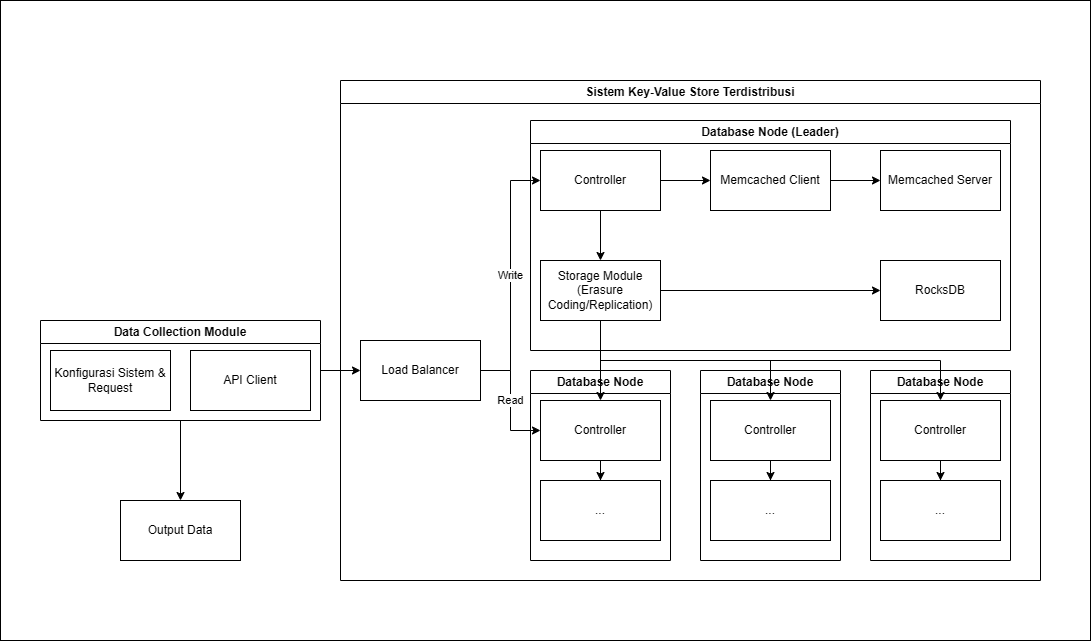
\includegraphics[width=0.95\textwidth]{resources/chapter-3/general-architecture.png}
    \caption{Struktur Data Collector}
    \label{fig:data-collector-structure}
\end{figure}